\documentclass[12pt]{report}
\usepackage[a4paper,margin=1in]{geometry}
\usepackage{setspace}
\usepackage{graphicx}
\usepackage{sectsty}
\usepackage{pdfpages}
% \usepackage{booktabs}
\usepackage[export]{adjustbox}
\usepackage{amssymb}
\usepackage{cancel}
\usepackage[numbered]{matlab-prettifier}
\usepackage{circuitikz}
\usepackage{xfrac}
\usepackage{lmodern}
\usepackage{multicol}
\usepackage{caption}
\usepackage{amsmath}
\usepackage{enumitem}

\usetikzlibrary{arrows}
\graphicspath{{images/}}
\usetikzlibrary{calc,patterns,angles,quotes}

\allsectionsfont{\centering}
\renewcommand\thesection{\arabic{section}}
\renewcommand{\thefootnote}{\arabic{footnote}}
\setcounter{tocdepth}{5}

\begin{document}

\input{titlepage}
\pagenumbering{roman}
{\tableofcontents\let\clearpage\relax\listoffigures}
\clearpage
\pagenumbering{arabic}
\newpage
\begin{flushleft}
% ---------------------------------------------------------------------------- %
\section{Conceptualize the Problem}
% ---------------------------------------------------------------------------- %

\begin{figure}[h]
  \begin{minipage}[c]{.4\textwidth}
  \usetikzlibrary{calc,patterns,angles,quotes}
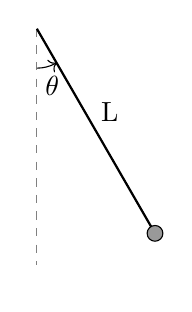
\begin{tikzpicture}
    % save length of g-vector and theta to macros
    \pgfmathsetmacro{\Gvec}{1.5}
    \pgfmathsetmacro{\myAngle}{30}
    % calculate lengths of vector components
    \pgfmathsetmacro{\Gcos}{\Gvec*cos(\myAngle)}
    \pgfmathsetmacro{\Gsin}{\Gvec*sin(\myAngle)}

    \coordinate (centro) at (0,0);
    \draw[dashed,gray,-] (centro) -- ++ (0,-3) node (mary) [black,below]{$ $};
    \draw[thick] (centro) -- ++(270+\myAngle:3) coordinate (bob);
    \pic [draw, ->, "$\theta$", angle eccentricity=1.5] {angle = mary--centro--bob};
    \draw (bob) -- (centro) node[midway, above]{~~~L};
    \filldraw [fill=black!40,draw=black] (bob) circle[radius=0.1];
\end{tikzpicture}

\end{minipage}%
\begin{minipage}[c]{.6\textwidth}
  The pendulumn system consists of two rigid bars attached at their ends by a linear spring.
\end{minipage}
% \caption{Conceptualization of the Dynamic System}
\end{figure}

\subsection{Constants and Assumptions}
\begin{tabular}{ll@{\hskip .75in}l}
 \multicolumn{1}{c}{Constants:} && \multicolumn{1}{c}{Assumptions:} \\
 Bar Mass: &$m$ = 0.25kg & Frictionless\\
 Bar Length: &$L$ = 0.5m & Released from Rest\\
 Gravity: &$g$ = 9.81$\sfrac{m}{s^2}$ &Rigid-Body Dynamics \\
 Linear Spring: \\
 \quad Spring Coefficient:& $k = 25~\sfrac{N}{m}$\\
 \quad Unstretched Length:& $L$ \\
\end{tabular}
\vspace{5ex}

We are asked to determine the following: \\
\begin{enumerate}
  \item The 6 Equations / 6 Unknowns for the system to solve for the Equations of Motion.
  \item Integrate the Equations of Motion using various initial conditions.
  \begin{enumerate}
    \item $\theta_o = \sfrac{\pi}{12}~rad, \quad \phi_o = \sfrac{\pi}{12}~rad$
    \item $\theta_o = \sfrac{-\pi}{12}~rad, \quad \phi_o = \sfrac{\pi}{12}~rad$
    \item $\theta_o = \sfrac{\pi}{36}~rad, \quad \phi_o = \sfrac{\pi}{12}~rad$
  \end{enumerate}
  \item Linearize the Equations of Motion assuming small angular positions and velocities
  (i.e. small angle approximation $\sin(x) \approx x,~\cos(x) \approx 1$)
  \begin{itemize}
    \item Determine the A matrix below.
  \end{itemize}
\end{enumerate}
\begin{equation}
\begin{bmatrix}
  \ddot{\theta} \\
  \ddot{\phi}
\end{bmatrix}
=
\begin{bmatrix}
A
\end{bmatrix}
\begin{bmatrix}
\theta \\
\phi
\end{bmatrix}
\nonumber
\end{equation}
\begin{enumerate}[resume]
  \item Find the natural frequencies of the system and their respective eigenvectors
  using the eigenvalues and eigenvectors of [A].
  \item Using information from (5), solve for the analytical solution to the
  linearized Equations of Motion and plot them for the initial conditions defined in (2).
\end{enumerate}
\newpage

% ---------------------------------------------------------------------------- %
\section{Free Body Diagram}
% ---------------------------------------------------------------------------- %
\begin{figure}[ht]
   \begin{minipage}[c]{.25\textwidth}
      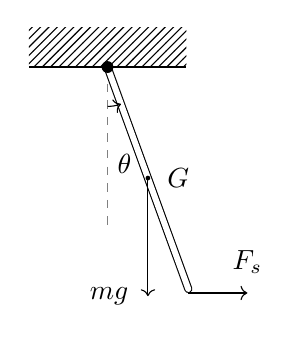
\begin{tikzpicture}

  \pgfmathsetmacro{\Gvec}{1.5}
  \pgfmathsetmacro{\myAngle}{20}

  \pgfmathsetmacro{\Gcos}{\Gvec*cos(\myAngle)}
  \pgfmathsetmacro{\Gsin}{\Gvec*sin(\myAngle)}

  \coordinate (centro) at (0,0);
  \draw[dashed,gray,-] (centro) -- ++ (0,-2) node (mary) [black,below]{$ $};
  \draw[double distance = .75mm,line cap=round] (centro) -- ++(270+\myAngle:3) coordinate (bob);
  \draw[->] (270+\myAngle:1.5) coordinate (g) -- ($(270+\myAngle:1.5) + (0,-1.5)$) coordinate (mg);
  \draw (mg) node[label=180:$mg$] {};
  \draw (g) node[label=east:$G$] {};
  \fill[black] (270+\myAngle:1.5) circle (0.03);
  \pic [draw,->, "$\theta$", angle eccentricity=2.5] {angle = mary--centro--bob};

  \fill[pattern = north east lines] ($ (centro) + (-1,0) $) rectangle ($ (centro) + (1,0.5) $);
  \draw[thick] ($ (centro) + (-1,0) $) -- ($ (centro) + (1,0) $);

  \fill[black] (centro) circle (0.075);

  (270+\myAngle:3) coordinate (bob2);

  \draw[->] ($ (bob) + (0,-.05) $) -- ++(0:.75) coordinate (fs);
  \draw (fs) node[label=north:$F_s$] {};

\end{tikzpicture}

   \end{minipage}%
   \begin{minipage}[c]{.5\textwidth}
     \hfill
     \begin{tabular}{rl}
     $F_s$:&Force onto bar by the spring\\
     $mg$:&Mass $\cdot$ gravity, weight of the bar\\
     $G$:&Center of gravity of each bar\\
     $\theta,~\phi$:& Angle of bar relative to vertical\\
   \end{tabular}
   \end{minipage}%
  \begin{minipage}[c]{.25\textwidth}
    \vspace{2.8ex}
    \hspace{2ex}
     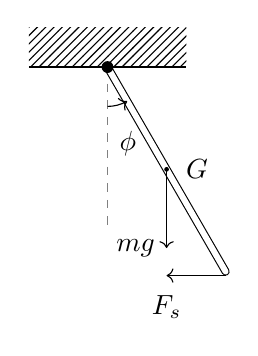
\begin{tikzpicture}

  \pgfmathsetmacro{\Gvec}{1.5}
  \pgfmathsetmacro{\myAngle}{30}

  \pgfmathsetmacro{\Gcos}{\Gvec*cos(\myAngle)}
  \pgfmathsetmacro{\Gsin}{\Gvec*sin(\myAngle)}

  \coordinate (centro) at (0,0);
  \draw[dashed,gray,-] (centro) -- ++ (0,-2) node (mary) [black,below]{$ $};
  \draw[double distance = .75mm,line cap=round] (centro) -- ++(270+\myAngle:3) coordinate (bob);
  \draw[->] (270+\myAngle:1.5) coordinate (g) -- ($(270+\myAngle:1.5) + (0,-1)$) coordinate (mg);
  \draw ($(mg) + (.1,0)$) node[label=180:$mg$] {};
  \draw (g) node[label=east:$G$] {};
  \fill[black] (270+\myAngle:1.5) circle (0.03);
  \pic [draw,->, "$\phi$", angle eccentricity=2] {angle = mary--centro--bob};

  \fill[pattern = north east lines] ($ (centro) + (-1,0) $) rectangle ($ (centro) + (1,0.5) $);
  \draw[thick] ($ (centro) + (-1,0) $) -- ($ (centro) + (1,0) $);

  \fill[black] (centro) circle (0.075);

  \draw[->] ($ (bob) + (0,-.05) $) -- ++(180:.75) coordinate (fs);
  \draw (fs) node[label=south:$F_s$] {};

\end{tikzpicture}

  \end{minipage}
\end{figure}

\subsection*{Acceleration Diagram}
\begin{figure}[ht]
   \begin{minipage}[c]{.25\textwidth}
      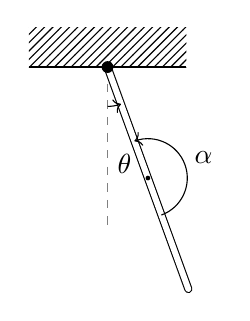
\begin{tikzpicture}

  \pgfmathsetmacro{\Gvec}{1.5}
  \pgfmathsetmacro{\myAngle}{20}

  \pgfmathsetmacro{\Gcos}{\Gvec*cos(\myAngle)}
  \pgfmathsetmacro{\Gsin}{\Gvec*sin(\myAngle)}

  \coordinate (centro) at (0,0);
  \draw[dashed,gray,-] (centro) -- ++ (0,-2) node (mary) [black,below]{$ $};
  \draw[double distance = .75mm,line cap=round] (centro) -- ++(270+\myAngle:3) coordinate (bob);
  % \draw[->] (270+\myAngle:1.5) coordinate (g) -- ($(270+\myAngle:1.5) + (0,-1.5)$) coordinate (mg);
  % \draw (mg) node[label=180:$mg$] {};
  \fill[black] (270+\myAngle:1.5) circle (0.03) coordinate (barcenter);
  \pic [draw,->, "$\theta$", angle eccentricity=2.5] {angle = mary--centro--bob};
  \pic [draw,->, "$\alpha$", angle eccentricity=1.5] {angle = bob--barcenter--centro};

  \fill[pattern = north east lines] ($ (centro) + (-1,0) $) rectangle ($ (centro) + (1,0.5) $);
  \draw[thick] ($ (centro) + (-1,0) $) -- ($ (centro) + (1,0) $);

  \fill[black] (centro) circle (0.075);

\end{tikzpicture}

   \end{minipage}%
   \begin{minipage}[c]{.5\textwidth}
     \begin{tabular}{rl}
     $\alpha$:& $\ddot{\theta},~\ddot{\phi}$ respectively\\
   \end{tabular}
   \end{minipage}%
  \begin{minipage}[c]{.25\textwidth}
    % \vspace{2.8ex}
    \hspace{2ex}
     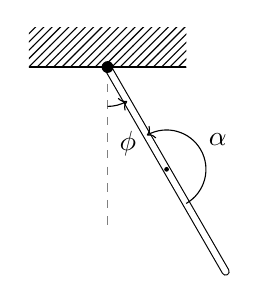
\begin{tikzpicture}

  \pgfmathsetmacro{\Gvec}{1.5}
  \pgfmathsetmacro{\myAngle}{30}

  \pgfmathsetmacro{\Gcos}{\Gvec*cos(\myAngle)}
  \pgfmathsetmacro{\Gsin}{\Gvec*sin(\myAngle)}

  \coordinate (centro) at (0,0);
  \draw[dashed,gray,-] (centro) -- ++ (0,-2) node (mary) [black,below]{$ $};
  \draw[double distance = .75mm,line cap=round] (centro) -- ++(270+\myAngle:3) coordinate (bob);
  % \draw[->] (270+\myAngle:1.5) coordinate (g) -- ($(270+\myAngle:1.5) + (0,-1)$) coordinate (mg);
  % \draw ($(mg) + (.1,0)$) node[label=180:$mg$] {};
  \fill[black] (270+\myAngle:1.5) circle (0.03) coordinate (bar2center);
  \pic [draw,->, "$\phi$", angle eccentricity=2] {angle = mary--centro--bob};
  \pic [draw,->, "$\alpha$", angle eccentricity=1.5] {angle = bob--bar2center--centro};

  \fill[pattern = north east lines] ($ (centro) + (-1,0) $) rectangle ($ (centro) + (1,0.5) $);
  \draw[thick] ($ (centro) + (-1,0) $) -- ($ (centro) + (1,0) $);

  \fill[black] (centro) circle (0.075);

\end{tikzpicture}

  \end{minipage}
\end{figure}

% ---------------------------------------------------------------------------- %
\section{Coordinate Frame}
% ---------------------------------------------------------------------------- %
\begin{center}
% \begin{figure}[ht]
%    \begin{minipage}[c]{.35\textwidth}
      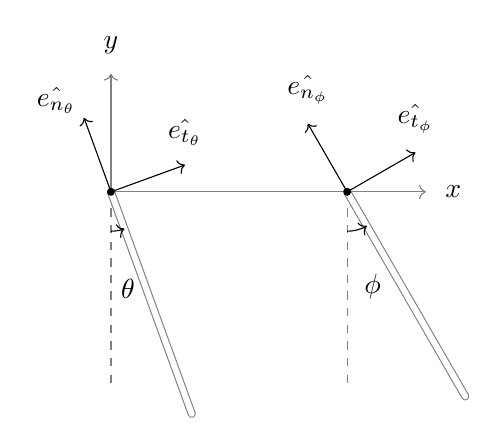
\begin{tikzpicture}

  \pgfmathsetmacro{\Gvec}{1.5}
  \pgfmathsetmacro{\myAngle}{20}

  \pgfmathsetmacro{\Gcos}{\Gvec*cos(\myAngle)}
  \pgfmathsetmacro{\Gsin}{\Gvec*sin(\myAngle)}

  \coordinate (centro) at (0,0);
  \draw[dashed,gray,-] (centro) -- ++ (0,-2.5) node (mary) [black,below] {};
  \draw[double distance = .75mm,line cap=round,gray] (centro) -- ++(270+\myAngle:3) coordinate (bob);

  \draw[->] (centro) -- ++(270+\myAngle:-1) coordinate (normL);
  \draw (normL) node[label={[label distance=-2mm]110:$\hat{e_{n_{\theta}}}$}] {};
  \draw[->] (centro) -- ++(20:1) coordinate (tanL);
  \draw (tanL) node[label=$\hat{e_{t_{\theta}}}$] {};
  \pic [draw,->, "${\theta}$", angle eccentricity=2.5] {angle = mary--centro--bob};



  \pgfmathsetmacro{\Gvec}{1.5}
  \pgfmathsetmacro{\myAngle}{30}

  \pgfmathsetmacro{\Gcos}{\Gvec*cos(\myAngle)}
  \pgfmathsetmacro{\Gsin}{\Gvec*sin(\myAngle)}

  \coordinate (centro) at (3,0);
  \draw[dashed,gray,-] (centro) -- ++ (0,-2.5) node (mary) [black,below] {};
  \draw[double distance = .75mm,line cap=round,gray] (centro) -- ++(270+\myAngle:3) coordinate (bob);

  \draw[->] (centro) -- ++(270+\myAngle:-1) coordinate (normR);
  \draw (normR) node[label=$\hat{e_{n_{\phi}}}$] {};
  \draw[->] (centro) -- ++(30:1) coordinate (tanR);
  \draw (tanR) node[label=$\hat{e_{t_{\phi}}}$] {};

  \pic [draw,->, "${\phi}$", angle eccentricity=2.5] {angle = mary--centro--bob};



  \draw [->,gray] (0,0) -- ++ (0:4) coordinate (x);
  \draw [->,gray] (0,0) -- ++ (90:1.5) coordinate (y);
  \draw (x) node[label=0:$x$] {};
  \draw (y) node[label=90:$y$] {};
  \fill[black] (centro) circle (0.05);
  \fill[black] (0,0) circle (0.05);
\end{tikzpicture}

%    \end{minipage}%
%    \begin{minipage}[c]{.65\textwidth}
%      \begin{tabular}{rl}
       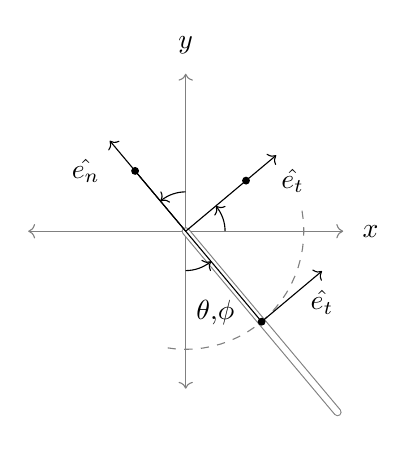
\begin{tikzpicture}

  \pgfmathsetmacro{\Gvec}{1.5}
  \pgfmathsetmacro{\myAngle}{40}

  \draw [->,gray] (0,0) -- ++ (0:2) coordinate (x);
  \draw [->,gray] (0,0) -- ++ (0:-2);
  \draw [->,gray] (0,0) -- ++ (90:2) coordinate (y);
  \draw [->,gray] (0,0) -- ++ (90:-2);
  \draw (x) node[label=0:$x$] {};
  \draw (y) node[label=90:$y$] {};

  \pgfmathsetmacro{\Gcos}{\Gvec*cos(\myAngle)}
  \pgfmathsetmacro{\Gsin}{\Gvec*sin(\myAngle)}

  \coordinate (centro) at (0,0);
  \coordinate (centro) -- ++ (0,-2.5) node (mary) {};
  \draw[double distance = .75mm,line cap=round,gray] (centro) -- ++(270+\myAngle:3) coordinate (bob);

  \draw[->] (centro) -- ++(270+\myAngle:-1.5) coordinate (norm);
  % \draw (norm) node[label=$\hat{e_n}$] {};
  \draw[->] (centro) -- ++(40:1.5) coordinate (tan);
  % \draw (tan) node[label=$\hat{e_t}$] {};
  \pic [draw,->, "$\theta\textrm{,}\phi$", angle eccentricity=2.2] {angle = mary--centro--bob};

  % \fill[black] (centro) circle (0.05);
  % \fill[black] (0,0) circle (0.05);


  \pic [draw,->, "$ $", angle eccentricity=2] {angle = x--centro--tan};
  \pic [draw,->, "$ $", angle eccentricity=2] {angle = y--centro--norm};

  \draw[gray,dashed,domain=10:-100] (centro) plot ({1.5*cos(\x)}, {1.5*sin(\x)});
  \fill[black] (centro) -- ++(40:1) circle (0.05) coordinate (co1);
  \draw (co1) node[label={[label distance=2mm]0:$\hat{e_t}$}] {};
  \fill[black] (centro) -- ++(130:1) circle (0.05) coordinate (co2);
  \draw (co2) node[label={[label distance=2mm]180:$\hat{e_n}$}] {};
  \fill[black] (270+\myAngle:1.5) circle (0.05);
  \draw[->] (270+\myAngle:1.5) -- ++(40:1) coordinate (tan2);
  \draw (270+\myAngle:1.5) -- (co2);
  \draw (tan2) node[label=-90:$\hat{e_t}$] {};

\end{tikzpicture}

%    \end{tabular}
%    \end{minipage}
% \end{figure}
% 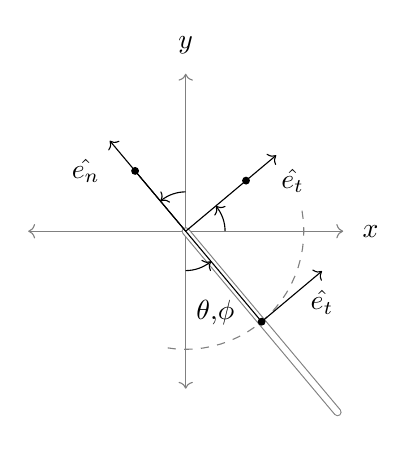
\begin{tikzpicture}

  \pgfmathsetmacro{\Gvec}{1.5}
  \pgfmathsetmacro{\myAngle}{40}

  \draw [->,gray] (0,0) -- ++ (0:2) coordinate (x);
  \draw [->,gray] (0,0) -- ++ (0:-2);
  \draw [->,gray] (0,0) -- ++ (90:2) coordinate (y);
  \draw [->,gray] (0,0) -- ++ (90:-2);
  \draw (x) node[label=0:$x$] {};
  \draw (y) node[label=90:$y$] {};

  \pgfmathsetmacro{\Gcos}{\Gvec*cos(\myAngle)}
  \pgfmathsetmacro{\Gsin}{\Gvec*sin(\myAngle)}

  \coordinate (centro) at (0,0);
  \coordinate (centro) -- ++ (0,-2.5) node (mary) {};
  \draw[double distance = .75mm,line cap=round,gray] (centro) -- ++(270+\myAngle:3) coordinate (bob);

  \draw[->] (centro) -- ++(270+\myAngle:-1.5) coordinate (norm);
  % \draw (norm) node[label=$\hat{e_n}$] {};
  \draw[->] (centro) -- ++(40:1.5) coordinate (tan);
  % \draw (tan) node[label=$\hat{e_t}$] {};
  \pic [draw,->, "$\theta\textrm{,}\phi$", angle eccentricity=2.2] {angle = mary--centro--bob};

  % \fill[black] (centro) circle (0.05);
  % \fill[black] (0,0) circle (0.05);


  \pic [draw,->, "$ $", angle eccentricity=2] {angle = x--centro--tan};
  \pic [draw,->, "$ $", angle eccentricity=2] {angle = y--centro--norm};

  \draw[gray,dashed,domain=10:-100] (centro) plot ({1.5*cos(\x)}, {1.5*sin(\x)});
  \fill[black] (centro) -- ++(40:1) circle (0.05) coordinate (co1);
  \draw (co1) node[label={[label distance=2mm]0:$\hat{e_t}$}] {};
  \fill[black] (centro) -- ++(130:1) circle (0.05) coordinate (co2);
  \draw (co2) node[label={[label distance=2mm]180:$\hat{e_n}$}] {};
  \fill[black] (270+\myAngle:1.5) circle (0.05);
  \draw[->] (270+\myAngle:1.5) -- ++(40:1) coordinate (tan2);
  \draw (270+\myAngle:1.5) -- (co2);
  \draw (tan2) node[label=-90:$\hat{e_t}$] {};

\end{tikzpicture}

\end{center}
% ---------------------------------------------------------------------------- %
\section{Sum of Forces}
% ---------------------------------------------------------------------------- %

\begin{equation}
  \sum Stuff
\end{equation}
Where: \\
~\\
\begin{tabular}{rl}
$\theta$:& Position of the left bar. \\
$\phi$:& Position of the right bar. \\
$\dot{\theta}$:& Angular velocity of the left bar. \\
$\ddot{\theta}$:& Angular acceleration of the left bar. \\
$\dot{\phi}$:& Angular velocity of the right bar. \\
$\ddot{\phi}$:& Angular acceleration of the right bar. \\
m, L, g: & Are constants; mass, length of each bar, and gravity, respectively
\end{tabular}
% ---------------------------------------------------------------------------- %
\section{Knowns and Unknowns} \label{knownsandunknowns}
% ---------------------------------------------------------------------------- %
\begin{tabular}{ll@{\hskip .75in}ll}
  \multicolumn{1}{c}{Knowns:} && \multicolumn{1}{c}{Unknowns:} \\
  Mass: &m = 0.142kg & String Tension: & T \\
  String Length: &L = 0.5m & Angular Acceleration: & $\ddot{\theta}$ \\
  Gravity: &g = 9.81$\sfrac{m}{s^2}$ \\
  State Variables: \\
  \quad Angular Velocity: &$\dot{\theta}$ & \\
  \quad Angular Acceleration:&$\ddot{\theta}$ & \\
\end{tabular}
\vspace{2ex}
\\

% ---------------------------------------------------------------------------- %
\section{Constraints}
% ---------------------------------------------------------------------------- %

% ---------------------------------------------------------------------------- %
\section{Solve for the Equations of Motion}
% ---------------------------------------------------------------------------- %

% ---------------------------------------------------------------------------- %
\section{Solve the Equations of Motion}
% ---------------------------------------------------------------------------- %

% ---------------------------------------------------------------------------- %
\section{Does it Make Sense?}
% ---------------------------------------------------------------------------- %
\subsection{Units}

\subsection{Magnitude}

\section{Appendix} \label{appendix}

\subsection{Attributions}

\onehalfspacing
\begin{tabular}{ll}
Jeffrey Chen & \\
Thorne Wolfenbarger & \\
Trey Dufrene & \\
Joint Effort &
\end{tabular}
\singlespacing

\subsection{Analytical Solution}

\subsection{Numerical Solution} \label{appendix:numerical}


\end{flushleft}
\end{document}
